% !TEX root = base.tex 

\chapter{Hematite Film Growth on Polycrystalline Substrates}
\label{ch:polycrystalline.growth}


\chintro{This chapter presents results for the growth of \ce{Fe2O3} films on polycrystalline \ce{SrTiO3} substrates. Film growth on polycrystalline substrates allows for interesting, high throughput explorations of orientation effects on film growth and photochemical activity. The polycrystalline substrate exposes a much wider range of orientation conditions than are available for single crystal substrates. Additionally, a single film deposition results in thousands of individual orientation relationships. By using electron backscatter diffraction, local orientation relationships can be observed and determined. }


\section{Film Growth and Orientation Data Collection}
\label{sec:poly.growth.experimental}


Following the deposition parameters in \sectionref{subsec:exp.pld}, a \SI{50}{\nano\meter} film was deposited on a polycrystalline \sto{} pellet.  The substrate pellet was prepared as described in \sectionref{subsec:exp.solidstate}. The substrate was approximately \SI{2}{\milli\meter} thick and \SI{8}{\milli\meter} in diameter. Depositions parameters were as described in \tableref{pldparameters}. After deposition, an area of the film was mapped using electron backscatter diffraction (\abbr{EBSD}). The film was polished away by hand using \SI{0.3}{\micro\meter} colloidal silica. The film and substrate were easily differentiated, as the film was red and the substrate was tan. Polishing was stopped when no more red material was visible on the surface of the pellet, after \texttildelow\SI{30}{\second}. The sample was returned to the \abbr{sem}, and the same area of the surface was mapped. The relatively large size of the polishing abrasive used to remove the film reduced the pattern quality of the diffraction patterns, however image acquisition parameters could be adjusted to obtain sufficient image quality (\abbr{IQ}) and confidence index (\abbr{CI}) parameters. The data was processed with one iteration of a grain dilation algorithm, and subsequently assigning a single average orientation to each grain. In the grain dilation cleanup method, points not belonging to an already identified grain (based on misorientation angle and grain size) are changed to the orientation of the nearest grain.  For this procedure, the minimum grain size was 5 pixels and the grain tolerance angle was 5\si{\degree}. The grain averaging procedure uses a tolerance angle to identify grains, and then assigns a single orientation to that grain, averaging the orientation of all points within the identified grain. The results of these two cleanup procedures are maps with clearly identified grains of a single orientation.


\begin{figure}
\begin{center}
	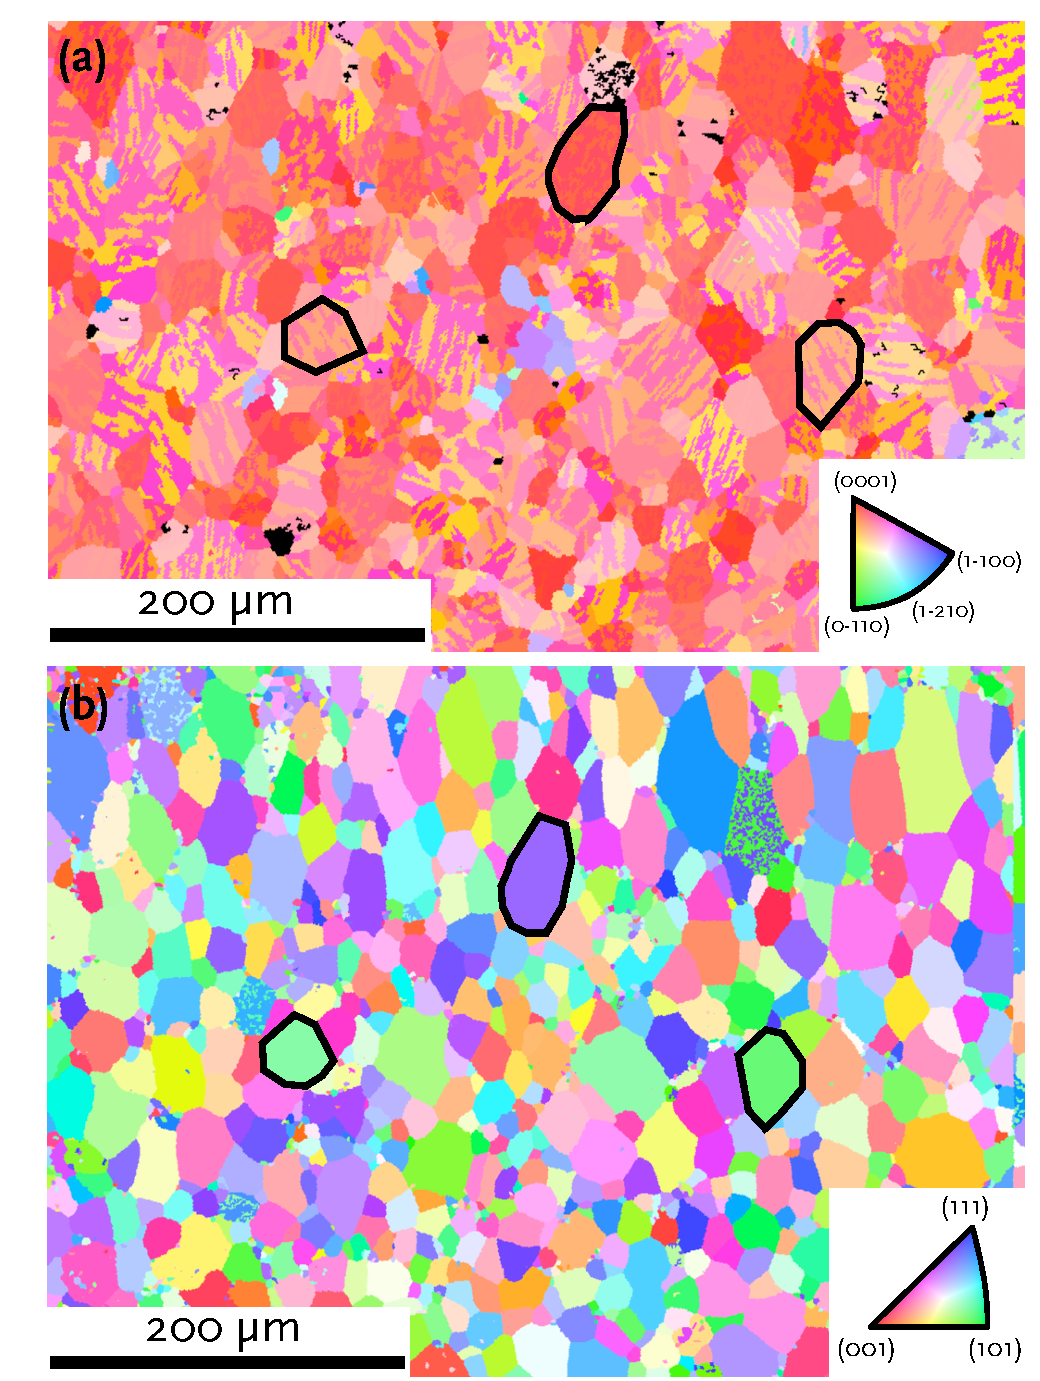
\includegraphics[width=\textwidth]{subfilmmaps.pdf}
		\caption[\abbr{EBSD} maps of film and substrate]{%
			\abbr{EBSD} maps of the same area of a \SI{50}{\nano\meter}
			\ce{Fe2O3} film on a polycrystalline \ce{SrTiO3} substrate.
			Outlined areas represent the same area of the sample.}
	\label{fig:subfilmmaps}
\end{center}
\end{figure}

The substrate and film maps are shown in \figureref{subfilmmaps}. The map in \figureref{subfilmmaps}(a) is the film, while \figureref{subfilmmaps}(b) depicts the the same area of the substrate after film removal. The outlined regions in each map represents pairs of film and substrate grains. For most substrate grains, a similar clearly distinguishable set of film grains can be outlined, with borders matching the shape of the corresponding substrate grain. In general, each substrate grain nucleates a set of film grains, often corresponding to two distinct orientations. Even film grains that appear to be a single red color are actually multiple film grains, as determined by the \abbr{EBSD} software. 
\begin{figure}
\begin{center}
	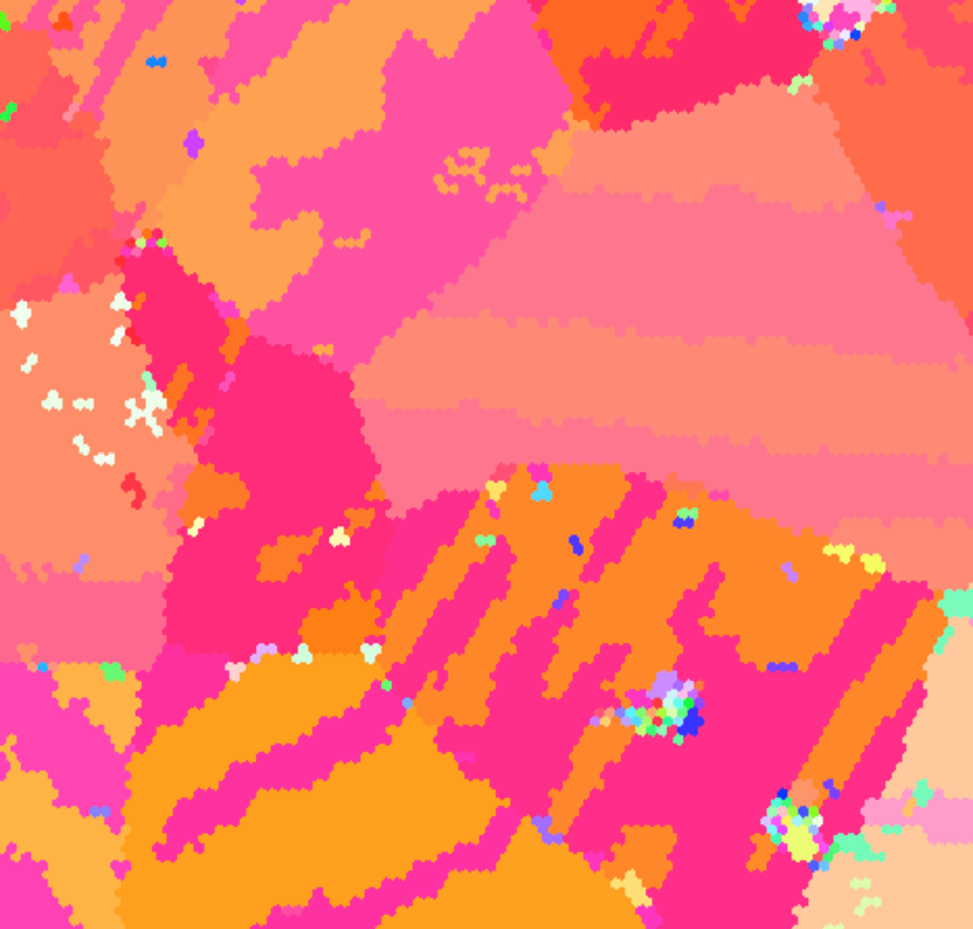
\includegraphics[width=0.4\textwidth]{zoommap.pdf}
		\caption[Detail of \abbr{EBSD} map]{%
			High resolution \abbr{EBSD} detail showing the lamellar
			structure of \ce{Fe2O3} film grains within a single substrate
			grain.}
	\label{fig:zoommap}
\end{center}
\end{figure}
%\sidefigure[Detail of \abbr{EBSD} map]{%
%	High resolution \abbr{EBSD} detail showing the lamellar
%	structure of \ce{Fe2O3} film grains within a single substrate
%	grain.
%	\label{fig:zoommap}
%	}{%
%	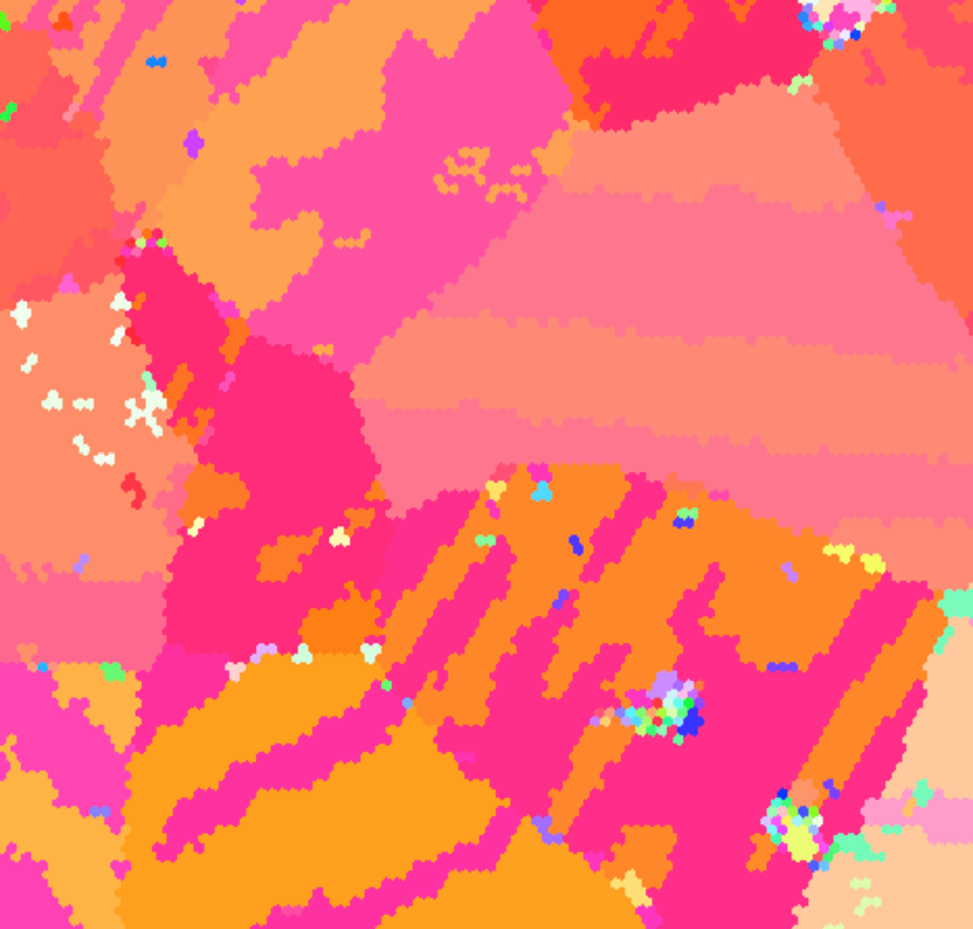
\includegraphics[width=\marginparwidth]{zoommap.pdf}
%}{-9} 
These sets of film grains typically appear in lamellar formations, shown in the high resolution scan detail in \figureref{zoommap}.

The colors used in inverse pole maps such as those presented in \figureref{subfilmmaps} represent the orientation of each point on the map. The orientation assignment for each color is determined using the color filled standard stereographic triangle. The substrate map represents grains representing the entire color space of the key, suggesting a random arrangement of orientations. Conversely, the inverse pole figure for the film shows grains that are varying shades red, orange, pink, and yellow. These colors represent film grains located near the (0001) orientation, which is represented by solid red on the inverse pole maps. This suggests that the film grains are all nearer each other in orientation compared to the substrate. This doesn't take into account differences between the film and substrate phases when describing the orientation of their respective grains. Because of its higher symmetry, the entire range of orientations of the cubic substrate can be represented in a smaller standard stereographic triangle than the hexagonal film material. The angle between the red, (001)-oriented and blue, (111)-oriented substrate grains (the maximum misorientation for cubic crystals) is \SI{54.7}{\degree}. For the hexagonal \feo, the angle between red grains and blue grains is \SI{90}{\degree}. 
\begin{figure}
	\begin{center}
	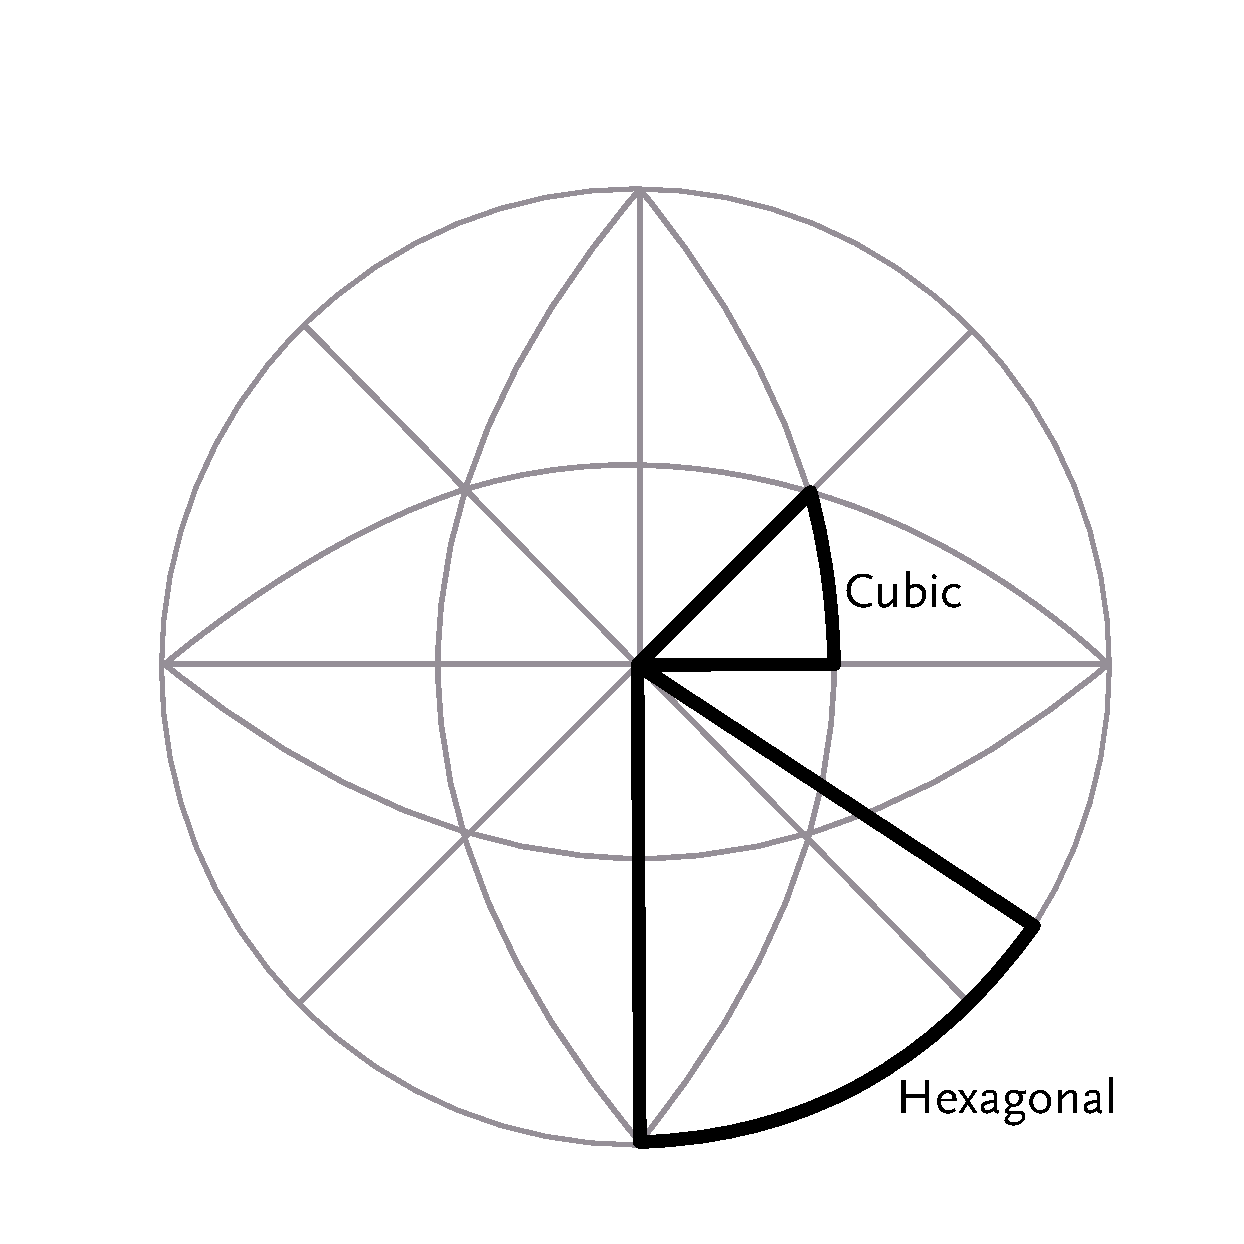
\includegraphics[width=0.5\textwidth]{stereotriangles.pdf}
		\caption[Relationship of stereographic triangles]{%
			Relationship of the standard stereographic triangles for hexagonal
			and cubic systems to each other and the complete stereographic 
			projection.}
	\label{fig:stereotriangles}
	\end{center}
\end{figure}
%\sidefigure[Relationship of stereographic triangles]{%
%	Relationship of the standard stereographic triangles for hexagonal
%	and cubic systems to each other and the complete stereographic 
%	projection.
%	\label{fig:stereotriangles}
%	}{%
%	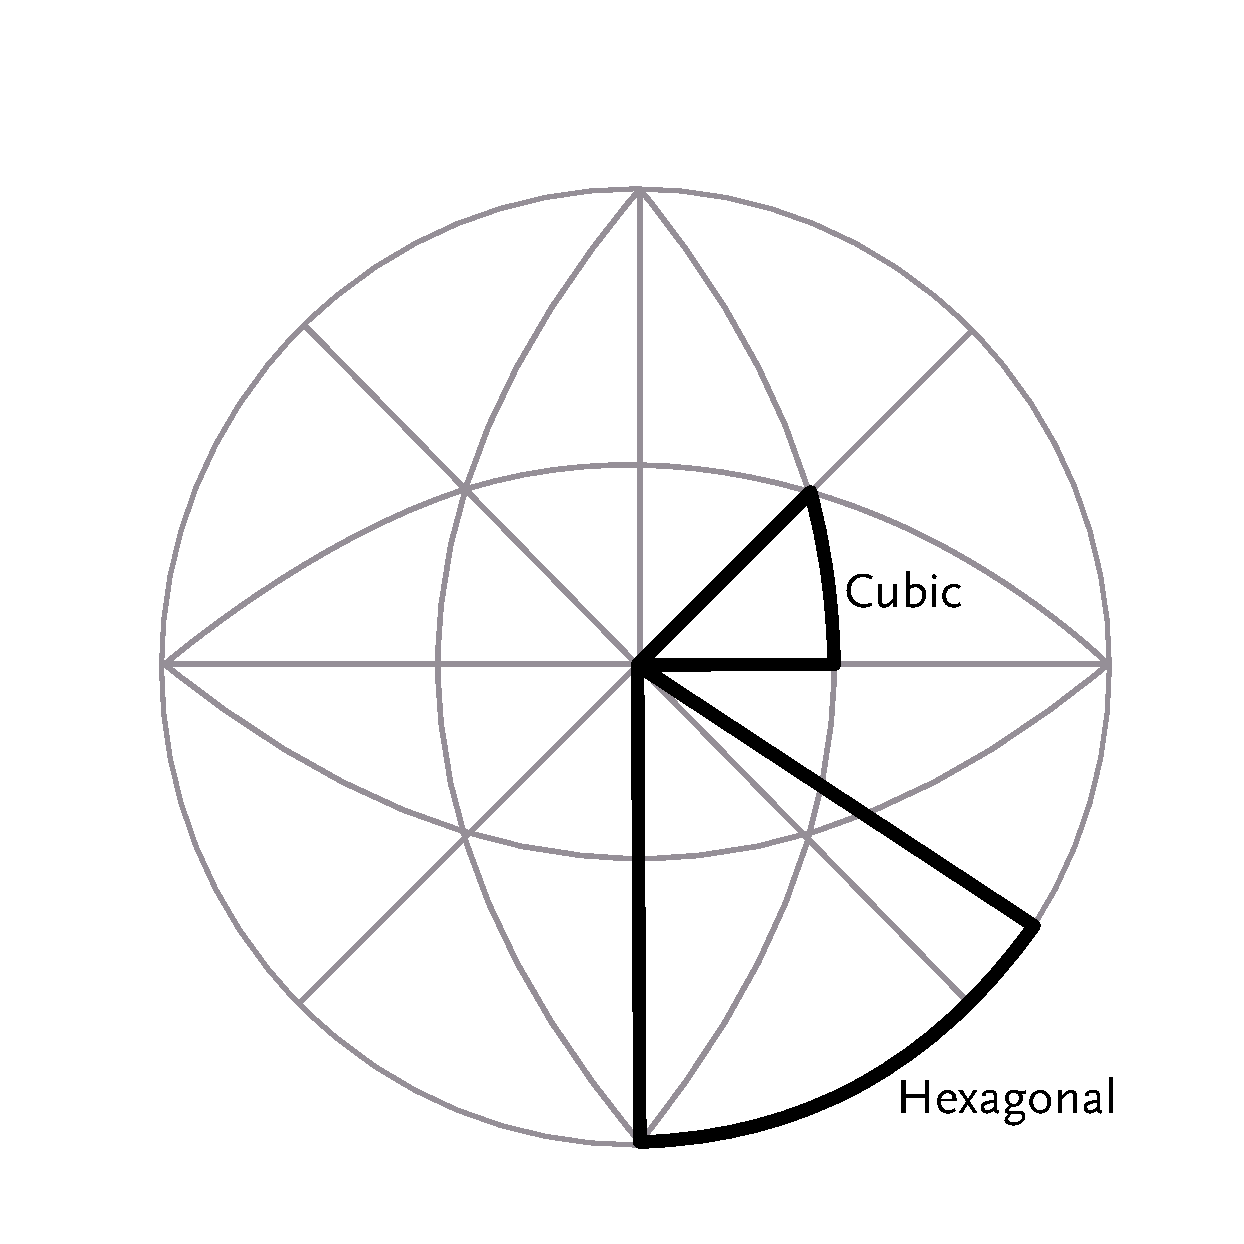
\includegraphics[width=\marginparwidth]{stereotriangles.pdf}
%}{-15}
\figureref{stereotriangles} shows the relationship of the cubic and hexagonal stereographic triangles to each other and the entire stereographic projection. The same color scale represents a wider set of orientations in the hexagonal system. As a result, a simple comparison of the color variance between these two images doesn't accurately reflect the differences in orientation spread for the two maps.


\section{Orientation Relationship Analysis}
\label{sec:poly.growth.orients}


For \ce{Fe2O3} films on single crystal \ce{SrTiO3} (001) substrates, the orientation relationship was \ce{Fe2O3}(0001)||\-\ce{SrTiO3}(111) for a significant portion of film grains (\texttildelow90\%), even though the \ce{SrTiO3} (111) direction was not the out of plane direction. It was hypothesized that a similar relationship could be determined for the substrate grains tilted away from the (111) direction on the polycrystalline substrate. The \ce{Fe2O3}(0001)||\ce{SrTiO3}(111) orientation relationship would persist, even for grains tilted away from (111) orientation. To test this hypothesis, data from these maps was exported in the form of a text file containing a single line for each identified grain of the scan. Each grain was assigned a unique number ID. This ID was included, along with the Euler angles corresponding to the angle of that grain.  The grain ID for each film grain was manually paired with the grain ID for its corresponding substrate grain. This was done through visible inspection of the maps depicted in Figure \ref{fig:subfilmmaps}. Only film grains that could clearly be assigned to a substrate grain were included in the pairing list. Because multiple film grains exist on a single substrate grain, in many cases multiple pairings exist for a single substrate grain. A program was then used to calculate the minimum angle between a film direction and a substrate direction, taking into account symmetry operations for the film and substrate crystal structures. 

117 such film/substrate pairs were analyzed to determine their orientation relationships. Because each substrate grain corresponds to multiple film grains, the 117 substrate grains represent 501 distinct film grains. \figureref{subfilmipfs} shows standard stereographic triangles for the film and substrate, with each point within the triangles representing a substrate or film grain used for orientation relationship calculations.
\begin{figure}
	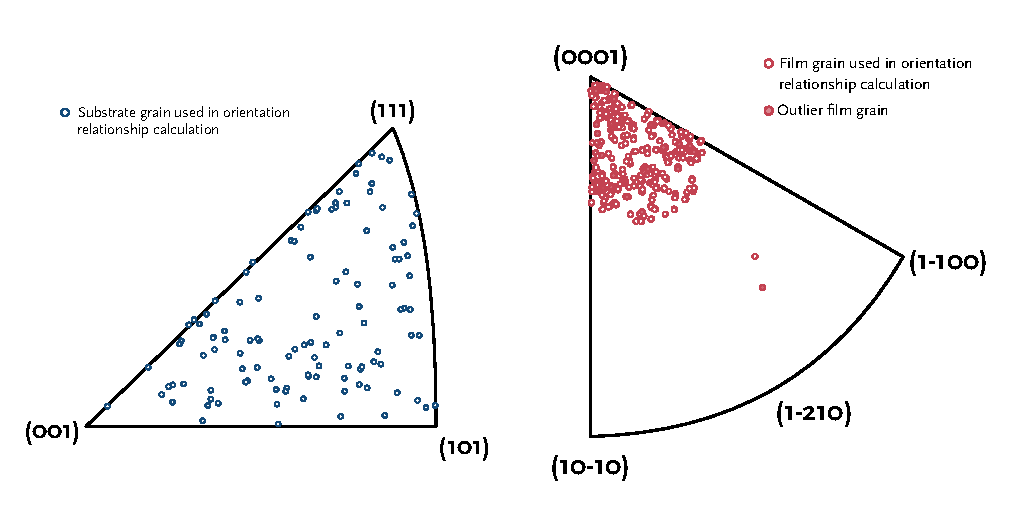
\includegraphics[width=\textwidth]{subfilmipfs.pdf}
		\caption[Orientation of film and substrate grains]{%
			Standard stereographic triangles representing the orientations
			of all grains in \figureref{subfilmmaps}. Each point on the 
			triangles represents a grain used for orientation calculations.}
	\label{fig:subfilmipfs}
\end{figure}
The substrate grains range widely over the entire area of the cubic standard stereographic triangle. The film grains are clustered near the (0001) point of the triangle. Once again, the same caveat as for the inverse pole maps comes into play. The angle between the (001) point and the edge for the cubic triangle ranges from \SI{45}{\degree} for the (101) corner and \SI{54.7}{\degree} for the (111) corner. Then angle between the (001) point and all edge points for the hexagonal triangle is \SI{90}{\degree}. The angular spread of the points represented in the film triangle is close to the same angular spread represented by the entire area of the cubic substrate triangle.
\begin{table}
	
	\begin{center}
\begin{tabular}{lr}
	
		Min &
		0.26 \\
		
		Q1 &
		1.86 \\
		
		Median &
		2.77 \\
		
		Q3 &
		3.64 \\
		
		Mean &
		4.22 \\
		
		Std. Dev. &
		6.50 \\
		
		Lower Fence &
		-3.46 \\
		
		Upper Fence &
		8.96 \\
		
	\end{tabular}

\end{center}	\caption[Statistical descriptors of orientation relationship data]{Statistical descriptors of \feo[0001]/\sto[111] orientation relationship data.}
	\label{tab:outofplanestats}


\end{table}

%\sidetable[Statistical descriptors of orientation relationship data]{%
%	Statistical descriptors of \feo[0001]/\sto[111] orientation relationship data.
%	\label{tab:outofplanestats}}{%
%	\vspace{-2in} %to move the table
%	\begin{tabular}{lr}
%	
%		Min &
%		0.26 \\
%		
%		Q1 &
%		1.86 \\
%		
%		Median &
%		2.77 \\
%		
%		Q3 &
%		3.64 \\
%		
%		Mean &
%		4.22 \\
%		
%		Std. Dev. &
%		6.50 \\
%		
%		Lower Fence &
%		-3.46 \\
%		
%		Upper Fence &
%		8.96 \\
%		
%	\end{tabular}
%}
When the angle between the substrate [111] direction and the film [0001] direction is calculated for the 501 identified pairs in these scans, the average angle between the substrate [111] and the film [0001] is \SI{4.22}{\degree}. If outliers, defined as
\begin{gather}
\text{Lower Outlier} < \text{Lower Fence} = Q_{1}-3(Q_{3}-Q_{1})\\
\text{Upper Outlier} > \text{Upper Fence}=  Q_{3}+3(Q_{3}-Q_{1})
\end{gather}
where $Q_{1}$ is the lower quartile, $Q_{3}$ is the upper quartile, and $Q_{3}-Q_{1}$ is the interquartile range, the average angle is \SI{2.62}{\degree}. \tableref{outofplanestats} lists the statistical descriptors of the orientation relationship calculations. For the majority of substrate/film pairs, the film c-axis grew parallel to the substrate [111] direction, regardless of that direction's angle away from the surface normal. This orientation relationship is labeled as the ``out of plane'' relationship, mirroring the results for film growth on single crystal (111) oriented \sto substrates.

The same orientation program was used to calculated the angle between the substrate [110] direction and the film [10\={1}0] direction. This proposed relation reflects observed alignment of the prismatic directions for films grown on single crystal substrates. The average angle between the calculated directions was \SI{2.45}{\degree}. By the same analogy to growth on \sto (111) substrates as for the \ce{Fe2O3}[0001]||\ce{SrTiO3}[111], this alignment of the film [10\={1}0] direction and the substrate [110] direction is labeled as the ``in plane'' relationship.

\begin{figure}

	\begin{center}
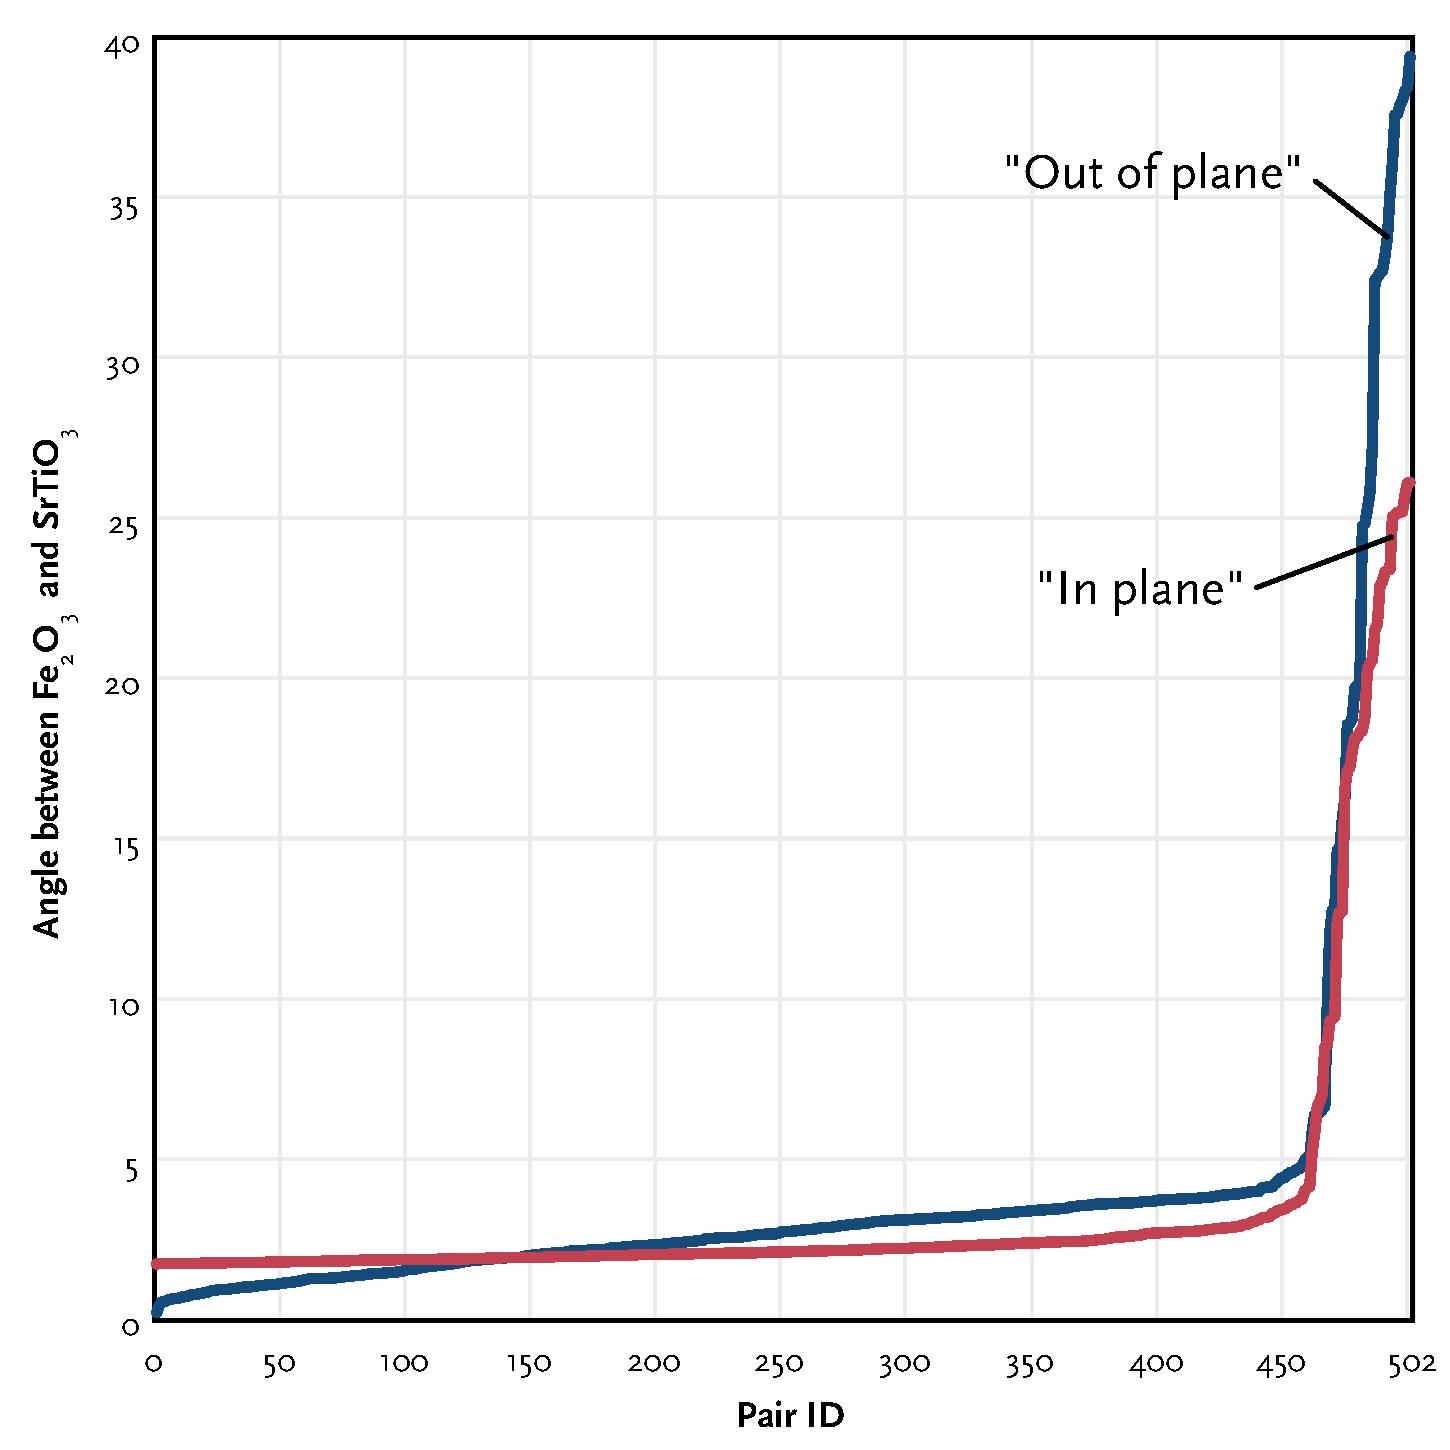
\includegraphics[width=0.6\textwidth]{orplots.pdf}
		\caption[Plot of film-substrate misorientations]{%
			Plot of the angle of misorientation between the film
			[0001] direction and the substrate [111] direction (out of plane, 
			blue) and the film [10\={1}0] direction and substrate [1\={1}0] 
			direction (red).}
	\label{fig:orplots}
\end{center}
\end{figure}
\figureref{orplots} tabulates the results for the orientation relationship calculations including all calculations for both alignments, the ``out of plane'' \ce{Fe2O3}[0001]||\ce{SrTiO3}[111] and the ``in plane'' \ce{Fe2O3}[10\={1}0]||\ce{SrTiO3}[1\={1}0]. For each plot, the majority of calculated relationships fall within the calculated upper fence. In general, points that were outliers (beyond the upper fence) for the ``out of plane'' relationship were also outliers for the ``in plane'' relationship. It is important to note here that the description of these points as outliers does not imply an error in data collection, or that the values calculated for these points don't represent the actual orientation relationships. This is shown here for six example substrate grains, on which outlier film orientation were found. Each identified film grain had consistent ``out of plane'' and ``in plane'' orientation relationships. These relationships are listed in \tableref{weirdgrains}.
\begin{table}
	
\centering
	\begin{tabular}{rrrr}

Substrate ID & Film ID &  [0001]$_{\text{Film}}$/[111]$_{\text{Sub}}$ (\degree)		&	[10\={1}0]$_{\text{Film}}$/[110]$_{\text{Sub}}$ (\degree)		\\

\cmidrule(lr){1-1}
\cmidrule(lr){2-2}
\cmidrule(lr){3-3}
\cmidrule(lr){4-4}

652		&	645		&	37.59	&	18.39	\\
		&	747		&	37.62	&	18.35	\\
		&	764		&	37.88	&	18.16	\\[4pt]
804		&	914		&	32.45	&	25.11	\\
		&	915		&	32.52	&	25.20	\\
		&	1020	&	32.67	&	25.21	\\
		&	922		&	32.73	&	25.22	\\[4pt]
828		&	1081	&	12.10	&	25.74	\\
		&	1089	&	12.80	&	26.11	\\
		&	1100	&	12.84	&	26.13	\\[4pt]
946		&	1409	&	33.78	&	8.59	\\
		&	1422	&	38.32	&	16.55	\\
		&	1393	&	38.43	&	12.53	\\
		&	1395	&	39.41	&	12.75	\\[4pt]
1468	&	2044	&	19.73	&	20.29	\\
		&	2058	&	19.79	&	20.48	\\
		&	2175	&	19.84	&	20.60	\\
	
	\end{tabular}

	\caption[Outlier misorientations]{%
		List of misorientation angles for grains that do not follow
		the observed orientation relationship between substrate and 
		film.}
	\label{tab:weirdgrains}
\end{table}
While within each grain, the orientation relationship is consistent, there is no single alignment that would describe all of these points. Substrate grains 652, 804, and 946 promoted films with the c-axis angled 30-40\degree from the substrate [111] direction. Grain 804 prompted film grains with a \texttildelow\ang{12} misorientation and grain 1468 a \texttildelow\ang{20} misorientation. Similarly, the ``in plane'' orientation relations are generally consistent within each substrate grain, but no single orientation relationship describes all the outlier grains.


\section{Discussion}
\label{sec:poly.growth.discussion}
		
		
Similar to the previously discussed growth of polycrystalline \ce{Fe2O3} films on \ce{SrTiO3} (001) substrates, the orientation relationship between the substrate and film is more complicated than the typical lattice parameter or interface plane view of epitaxy. A 2\textsc{d} description of the lattice matching wouldn't necessarily predict the consistent orientation relationship seen over a wide range of substrate orientations. Similarly, a description of the orientation relationship relying solely on out of plane and in plane vectors in the sample reference frame doesn't show the underlying consistent orientation relationship for these films on polycrystalline substrates. If the conventional sample normal vector were to be used to describe each substrate grain orientation relationship, the result would be 117 different orientation relationship descriptions, rather than the one consistent descriptor from the lattice reference frame used here to describe the majority of film-substrate pairs.

Across wide ranges of substrate orientations, the orientation relationship of the film [0001] and [10\={1}0] directions aligned with the substrate [111] and [1\={1}0] directions respectively. This relationship matches that observed for films on (111)-oriented single crystal substrates, as well as for 2 of the observed classes of film grains on (001)-oriented single crystal substrates (the purple and white partitions reported in \sectionpageref{subsubsec:single.growth.purplewhite}.) Based on single crystal substrate results, grains oriented very near the (111) orientation would be expected to show this relationship from a simple 2\textsc{d} lattice parameter analysis.\footnote{See \sectionpageref{sec:single.growth.111}.}

An analysis of the close packed (eutactic)\cite{OKeeffe:1977vx} crystal directions of the film and substrate leads to a proposed mechanism for the persistent orientation relationship. The hematite structure is a hexagonal close packed (hcp) network of oxygen atoms, with iron atoms filling \slantfrac{2}{3} of the interstitial sites. The close packed oxygen plane is the (0001) plane, and the close packed direction within this plane is the <1\={1}00> family of directions. The \ce{SrTiO3} substrate is a cubic close packed (ccp) network of \ce{SrO3} atoms, with titanium atoms in \slantfrac{1}{4} of the octahedral interstitial sites. The close packed planes are the \{111\} family of planes, and the close packed directions within that plane are <1\={1}0>. The close placed planes, \ce{Fe2O3}[0001] and \ce{SrTiO3}[111], are also the planes that represent the ``out of plane'' orientation relationship. The close packed planes are consistently aligned between substrate and film grains. The close packed directions match the determined ``in plane'' orientation relationship. For \ce{Fe2O3} films grown on \ce{SrTiO3} substrates, the close packed network is aligned between film and substrate over a wide spread of substrate orientation conditions.

It is noted that the use of multiple film/substrate pairs for each substrate grain affects the validity of the statistical analysis of the data. Because each substrate grain resulted in an average of \texttildelow{}4 calculated orientation relationships, much of the data can be thought to represent redundant information. Each additional film grain doesn't represent an entirely unique substrate-grain pair. Despite this, the decision was made to include all data for orientation relationship calculations. In all cases, at least two different film orientation bins were observed on a single substrate grain, regardless of the actual number of film grains. Manually selecting just one of these orientation families could leave out important differences between the film grains. Additionally, in some cases, some film grains showed a very small misorientation between the selected substrate and film directions, while other film grains \emph{on the same substrate grain} showed a much larger misoriention. If only one film grain was selected for each substrate grain, this effect could be amplified or completely missed, depending on the random selection of film grain. Finally, the inclusion of all film/substrate orientation calculations provides a higher sample size. The larger sample size will result in a more accurate statistical depiction of the total population, so long as the limitations here are understood.

The use of polycrystalline substrates and electron backscatter diffraction mapping for film growth analysis represents a technical step forward. The combination of these techniques, called combinatorial substrate epitaxy (\abbr{CSE}), allows for high throughput studies of film growth on high and low index orientations. With the inclusion of a local probe property measurement technique, such as the marker reactions used in this document or \abbr{AFM} probing of electronic properties, effects of orientation on material properties can be investigated. Using \abbr{CSE}, a single film deposition results in hundreds of individual substrate/film pairs. Each of these pairs can be thought to represent a single growth experiment. Even if single crystal substrates could be obtained in all of these orientations, the deposition time alone would prohibit such wide-ranging epitaxy analyses.


\section{Conclusion}
\label{sec:poly.growth.conclusion}

\ce{Fe2O3} films were grown on polycrystalline \ce{SrTiO3} substrates. The film-substrate orientation relationship was consistent for most substrate grains. The close packed (eutactic) network of the film grains aligned with that of the substrate grains. For the \ce{Fe2O3}/\ce{SrTiO3} system, this results in an arrangement described by \ce{Fe2O3}[0001]||\ce{SrTiO3}[111] and \ce{Fe2O3}[10\={1}0]||\ce{SrTiO3}[1\={1}0]. This orientation relationship is the same as observed for films on (111)-oriented single crystal substrates, however in this case, the (111) plane is not parallel to the surface for most substrate crystallites. The eutactic orientation relationship persisted, even when the close packed plane was tilted away from the surface normal.

